\section{SiPM Power Supply}

One of the goals we want to achieve with the tracking plane is a homogeneous and stable gain of all the SiPMs. For that reason from the beginning we have developed our own SiPM power supply, which provides a very clean bias voltage and is able to compensate the temperature variations in order to keep the SiPM gain. After operating the SiPM power supply during long time in NEXT-DEMO, we decide to improve it and add some missing features:

\begin{itemize}
\item Communication and control over Ethernet.
\item Current measurement.
\item Cost reduction.
\end{itemize}

\subsection{Electronic design}

Now we have a new design that offers similar specifications to the old power supply but it reduces costs and has more and better functionalities. In the figure \ref{fig:esq} is shown the scheme of the main hardware.

\begin{figure}[ht]
\centering 
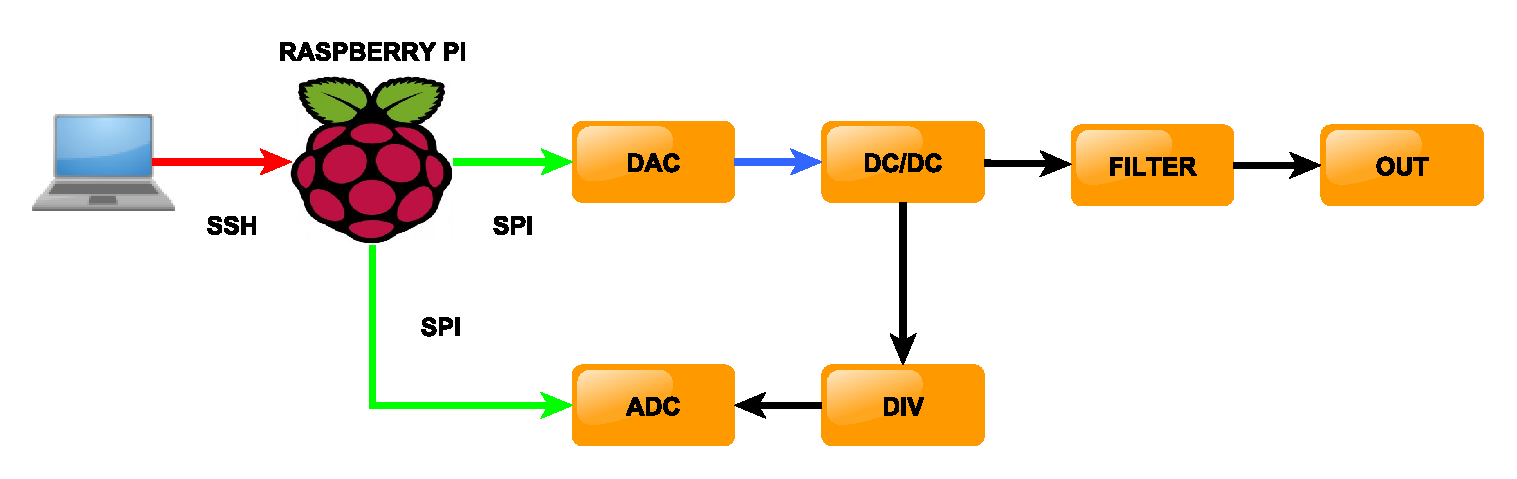
\includegraphics[width=.8\columnwidth]{5ch.pdf} 
\caption{\textit{Diagram}} 
\label{fig:esq} 
\end{figure}

The most important stage in the power supply is the DC/DC converter. This device is responsible for supplying the SiPMs bias, which will be around $70-74\ V$. We found a new DC/DC, the \emph{LT3482}, which is smaller and has an internal switch to limit the current. The DC/DC with a filter on the output gives the same result as the old one, but costs $5$ \euro\ as opposed to the $70$ \euro\ cost of the previous DC/DC.

The new DAC and ADC have higher resolution, but at a similar cost to the old ones. The DAC chosen is the \emph{AD5360} which has $16$-bit resolution permitting steps of about $1\ mV$ at the output of the DC/DC converter.  Moreover, the ADC is the \emph{LTC2418} and has $23$-bit resolution that offers $0,34\ mV$ of resolution to measure the output. Both devices have $16$ independent channels and SPI communication with the microcomputer.

For the output calibration we have tested several options, and we have finally chosen the use of external measurement equipment (\emph{Keathley} picoammeter). This method takes more time; however is cheaper than the others and can be automated.

The old microcontroller is very easy to program and we are experienced at this, but it has many limitations that prevent us from using the new power supply efficiently. The main problem is that it does not have by default an Ethernet port to communicate with other equipment via TCP/IP, and does not have internal memory. Without internal memory permanent communication with an additional PC is necessary, and if this communication is lost the measured data will be lost. For this reason we searched for an alternative.

\begin{figure}[ht]
\centering 
\includegraphics[width=0.6\columnwidth]{rasp} 
\caption{\textit{Raspberry Pi}} 
\label{fig:rasp} 
\end{figure}

The chosen alternative is the \emph{Raspberry Pi} (figure \ref{fig:rasp}), that is a credit card sized single-board microcomputer, which includes a $700\ MHz$ processor, \emph{VideoCore IV GPU}, and $512$ megabytes of RAM memory.  It uses an SD card for booting and data storage. Furthermore it costs less than the previous one.

The last hardware modification is the replacement of the old monochrome ASCII display by a $3.2"$ touchscreen, which will be placed on the front panel of a $3U$ box for rack mounting.

\subsection{Software characteristics}

There are improvements in the communication of the power supply. We decided to use stronger communication to control and monitor the power supply. The communication chosen is Secure Shell (SSH), which is a cryptographic network protocol for secure data communication. In addition we have Secure copy or SCP, which is a mean of securely transferring computer files based on the SSH protocol.
We have programmed an interface with SSH on LabVIEW and various scripts in the microcomputer of the power supply can be invoked with it; these are responsible for changing any internal parameter of the power supply.
The power supply can also be controlled or monitored easily using any computer with SSH or SCP protocols. The internal program is totally independent of these communications and has been prepared to prevent any error while working in stand-alone mode.

\begin{figure}[ht]
\centering
\subfloat[\textit{Single channel menu}]{\includegraphics[width=.28\columnwidth]{screen1}\label{fig:screen1}}
\hspace{20mm}
\subfloat[\textit{Main menu}]{\includegraphics[width=.28\columnwidth]{screen2}\label{fig:screen2}} \\
\caption{\textit{Touchscreen menu examples}}
\label{fig:screen}
\end{figure}

Independently of the Ethernet control, the power supply can be controlled, monitored and any parameter can be adjusted physically, using a small touchscreen which is shown on figures \ref{fig:screen1} and \ref{fig:screen2}.

The microcomputer generates reports in blocks of 24 hours with all the parameters (voltage, current and temperature), and with any error or unusual event that may have occurred. These parameters can be taken once a day or whenever needed using LabVIEW or any computer with SSH or SCP. In any case the reports will be stored in the internal memory of the power supply. 

The output voltage is adjusted continuously by an autocalibration algorithm, and the rise and fall slopes can be adjusted for slow bias polarization. These ramps appear on figure \ref{fig:ramp}, adjusted for a voltage slope of $10\ V/s$.

\begin{figure}[ht]
\centering
\subfloat[\textit{Rise ramp}]{\includegraphics[width=.49\columnwidth]{rise_mod}}
\subfloat[\textit{Fall ramp}]{\includegraphics[width=.49\columnwidth]{fall_mod}\label{fig:ipsum}} \\
\caption{\textit{Programmable rise and fall voltage ramp (10V/s)}}
\label{fig:ramp}
\end{figure}

As the old SiPM power supply, each channel provides the bias voltage for a full DICE-Board, where the $64$ SiPMs have the same gain at a fixed voltage. The temperature sensor placed on every DICE-Board is read by the SiPM power supply, so the voltage of each channel is modified to compensate the temperature variations, and keeps the SIPMs gain stable.

Also an overcurrent protection has been implemented, so if the current reaches a dangerous level, the affected channel is switched off automatically and a message is sent to the Slow Control system.

All parameters can be configured at any time, and easily, using SSH communication or the touchscreen menus.

\subsection{Results}
The 5-channel power supply, shown on the figure \ref{fig:5chan}, was assembled, and the code was updated to allow more user options and to introduce internal checks that verify the correct functionality of the power supply. These checks act and report if something bad happens. This prototype has been tested in NEXT-DEMO over a long period of time. It communicates reliably and runs correctly.

At first, we decided to construct $6U$ rack power supplies with $32$ channels, but as we have some space in the $3U$ front-end crate we decided to do one power supply of $16$ channels per front-end rack (each rack of the crate has $12$ frond-ends). This will simplify all the connexions and will be easier to control for the user. However, this design has  increased the price by $600$\euro\ for NEW and $2000$\euro\ for NEXT-100.

The 16-channel power supply for NEW has 2 boards with 8 channels and a supply board, the $3U$ rack power supply is shown on figure \ref{fig:16chan}. The code was updated and several improvements were made from the earlier prototype of $5$ channels. The new 16-channel source checks the internal temperature of the cards and incorporates an automatic shutdown protection if any internal overheating occurs. 

\begin{figure}[ht]
\centering
\subfloat[\textit{16 channels power supply}]{\includegraphics[height=.45\textwidth]{16_Channels_power_supply}\label{fig:16chan}} 
\hspace{15mm}
\subfloat[\textit{Prototype of 5 channels}]{\includegraphics[height=.35\textwidth]{3d_final}\label{fig:5chan}} \\
\caption{\textit{SiPM power supply prototype to be debugged on NEXT-DEMO}}
\end{figure}

The main specifications of the SiPM power supply are:

\begin{itemize}

\item Input voltage $\pm 12V$.
\item Maximum output current $5mA$ per channel.
\item Power consumption $5W (typ)$ and $29W (max)$.
\item Voltage range $0-85\ V$ with $1\ mV$ precision.
\item Measurement resolution $1/3\ mV$.
\item Low output noise (less than $4\ mVpp$).
\item Controlled rise and fall slopes.
\item Autocalibration algorithm.
\item Measurement of current with maximum error of $12\ \mu A$.
\item Temperature measurement and voltage compensation for gain stabilization.
\item Overheat protection, automatic off.
\end{itemize}

The output noise and long term stability have been measured with very good results. The voltage output, once calibrated, remains stable along weeks of operation with a precision of $1\ mV$. About the noise, as can be seen on the figure \ref{fig:noise}, normally is less than $1	\ mVpp$; but has some random peaks up to $4\ mV$ that can be seen with display persistence.

\begin{figure}[ht]
\centering
\subfloat[\textit{Single measurement}]{\includegraphics[height=.32\textwidth]{noise_71,15mod}}\label{fig:cont}
\hspace{5mm}
\subfloat[\textit{Continuous measurement with display persistence}]{\includegraphics[height=.32\textwidth]{noise_71,15Vmod}\label{fig:single}}

\caption{\textit{Noise in the output with $71.15\ V$}}
\label{fig:noise}
\end{figure}

By now, the 16-channel source is doing stability tests because the microprocessor manufacturers changed their model. The new model has some incompatibility with libraries designed and we modified the code. Because of these changes, the source must rerun time to debug the code, that it was verified on the $5$ channels prototype.

We will need $3$ of these power supplies to provide the bias voltage for the full NEW tracking plane, so $4$ of them are being produced to have a spare available.

About the cost per channel, it has been reduced by a factor $5$ compared with the old power supply.% A design requirement of the front-end has involved a increase of the price of the SiPMs power supply . We need to use expensive connectors and cable for connection between the power supply of SiPM and front-end . %The estimated cost for a $16$ channel SiPM power supply is $800$\euro, and the cables and connectors of it is $1450$\euro. We will need $3$ of these power supplies to provide the bias voltage for the full NEW tracking plane.

%-----------------------------------------------------------------




